%%%%%%%%%%%%%%%%%%%%%%%%%%%%%%%%%%%%%%%%%%%%%%%%%%%%%%%%%%%%%%%%%%%%%%%
%%%%%%%%%%%%%%%%%%%%%%%%%%%%%%%%%%%%%%%%%%%%%%%%%%%%%%%%%%%%%%%%%%%%%%% 
%%%%%%%%%%%       								 Preamble				         	                                                        %%%%%%%%%% 
%%%%%%%%%%%%%%%%%%%%%%%%%%%%%%%%%%%%%%%%%%%%%%%%%%%%%%%%%%%%%%%%%%%%%%% 
%%%%%%%%%%%%%%%%%%%%%%%%%%%%%%%%%%%%%%%%%%%%%%%%%%%%%%%%%%%%%%%%%%%%%%% 
\documentclass[10pt]{beamer}
\usepackage{setspace}
\usepackage{color}
\usepackage{amsmath,lmodern}
\usepackage{hyperref}
\usepackage{graphicx}
\usepackage{multirow}
\usepackage{tikz}
\usetikzlibrary{fit,shapes.misc}
\usepackage{pdflscape}
\usepackage{amsmath}
\usepackage{lscape}
\usepackage{multirow}
\usepackage{enumerate}
\usepackage{mathtools}
\usepackage{epstopdf}
\usepackage{pdfpages}
\usepackage{bm}
\usepackage{appendixnumberbeamer}
\usepackage{color,soul}
\usepackage{grffile}
\usepackage{float}
\usepackage{relsize}
\usepackage{tcolorbox}
\newcounter{nodemarkers}
\usepackage{tikz}
\newcommand{\toplinesmall}{%
  \tikz[remember picture,overlay] {%
    \draw[blue,thick] ([yshift=-1cm, xshift=.9cm]current page.north west)
             -- ([yshift=-1cm,xshift=3.6cm]current page.north west);}}
             
\newcommand{\toplinemedium}{%
  \tikz[remember picture,overlay] {%
    \draw[blue,thick] ([yshift=-1cm, xshift=.9cm]current page.north west)
             -- ([yshift=-1cm,xshift=6.2cm]current page.north west);}}
 
 \newcommand{\toplinelarge}{%
  \tikz[remember picture,overlay] {%
    \draw[blue,thick] ([yshift=-1cm, xshift=.9cm]current page.north west)
             -- ([yshift=-1cm,xshift=8.9cm]current page.north west);}}           
             
 \newcommand{\toplinexlarge}{%
  \tikz[remember picture,overlay] {%
    \draw[blue,thick] ([yshift=-1cm, xshift=.9cm]current page.north west)
             -- ([yshift=-1cm,xshift=12cm]current page.north west);}}                       
             
\setbeamertemplate{footline}
{
  \leavevmode%
  \hbox{%
  \begin{beamercolorbox}[wd=.333333\paperwidth,ht=2.25ex,dp=1ex,center]{author in head/foot}%
    \usebeamerfont{author in head/foot}{\textcolor{blue}{ECON712}}
  \end{beamercolorbox}%
  \begin{beamercolorbox}[wd=.333333\paperwidth,ht=2.25ex,dp=1ex,center]{title in head/foot}%
    \usebeamerfont{title in head/foot}{\textcolor{blue}{Winter 2026}}
  \end{beamercolorbox}%
  \begin{beamercolorbox}[wd=.333333\paperwidth,ht=2.25ex,dp=1ex,right]{date in head/foot}%
    \usebeamerfont{date in head/foot}{\textcolor{blue}{Lecture 4 \: \: \: \: \: \: \: }
    \insertframenumber{} / \inserttotalframenumber\hspace*{2ex}} 
  \end{beamercolorbox}}%
  \vskip0pt%
}
\newtheorem{proposition}[theorem]{Proposition}

\newcommand\marktopleft[1]{%
    \tikz[overlay,remember picture] 
        \node (marker-#1-a) at (-0.2,1.2ex) {};%
}
\newcommand\markbottomright[1]{%
    \tikz[overlay,remember picture] 
        \node (marker-#1-b) at (0.16,-1ex) {};%
    \tikz[overlay,remember picture,thick,inner sep=4pt]
        \node[draw,rectangle,rounded corners, blue, fit=(marker-#1-a.center) (marker-#1-b.center)] {};%
}

\setbeamertemplate{caption}{\raggedright\insertcaption\par}
\setbeamertemplate{itemize items}[ball]
\setbeamertemplate{itemize subitem}[triangle]
\setbeamertemplate{itemize subsubitem}[triangle]
\tcbset{colframe=white,colback=white,nobeforeafter}
\beamertemplatenavigationsymbolsempty
\addtobeamertemplate{frametitle}{\vspace*{0.19cm}}{\vspace*{0cm}}


%%%%%%%%%%%%%%%%%%%%%%%%%%%%%%%%%%%%%%%%%%%%%%%%%%%%%%%%%%%%%%%%%%%%%%%
%%%%%%%%%%%%%%%%%%%%%%%%%%%%%%%%%%%%%%%%%%%%%%%%%%%%%%%%%%%%%%%%%%%%%%% 
%%%%%%%%%  									    Define Title									                                       %%%%%%%%%
%%%%%%%%%%%%%%%%%%%%%%%%%%%%%%%%%%%%%%%%%%%%%%%%%%%%%%%%%%%%%%%%%%%%%%%
%%%%%%%%%%%%%%%%%%%%%%%%%%%%%%%%%%%%%%%%%%%%%%%%%%%%%%%%%%%%%%%%%%%%%%% 
\title{ECON 712: Applied Econometrics} 
\author{Lecture 4: Regression Fundamentals: Algebraic Properties of OLS}
\date{}
\AtBeginSection[]
{
 \begin{frame}<beamer>
 \tableofcontents[currentsection]
 \end{frame}
}
%%%%%%%%%%%%%%%%%%%%%%%%%%%%%%%%%%%%%%%%%%%%%%%%%%%%%%%%%%%%%%%%%%%%%%%
%%%%%%%%%%%%%%%%%%%%%%%%%%%%%%%%%%%%%%%%%%%%%%%%%%%%%%%%%%%%%%%%%%%%%%% 
%%%%%%%% 						     				Document								                                                %%%%%%%%
%%%%%%%%%%%%%%%%%%%%%%%%%%%%%%%%%%%%%%%%%%%%%%%%%%%%%%%%%%%%%%%%%%%%%%%
%%%%%%%%%%%%%%%%%%%%%%%%%%%%%%%%%%%%%%%%%%%%%%%%%%%%%%%%%%%%%%%%%%%%%%% 
\begin{document}
\setbeamercovered{transparent}

\begin{frame}
\maketitle
\end{frame}



\section{Multiple Linear Regression}

\begin{frame}
\frametitle{\: \: \: Multiple Regression: Matrix Form} 
\toplinelarge
\begin{itemize}
\item We are going to write the Multiple Regression Equation with $k$ regressors and $n$ observations as:
\begin{eqnarray*}
\underset{n \: X \: 1}{\bm{y}}=\bm{X} \underset{k \: X \: 1}{\bm{\beta}}+\underset{n \: X \: 1}{\bm{u}}
\end{eqnarray*}
where

\begin{eqnarray*}
\underset{n\: X \: k}{X}=
  \begin{bmatrix}
    \bm{X_1}\\
    \bm{X_2} \\
     \vdots \\
    \bm{X_n}\\
  \end{bmatrix}
=
 \begin{bmatrix}
     x_{11} & x_{12} & \cdots & x_{1k} \\
    x_{21} & x_{22} & \cdots & x_{2k} \\
     \vdots    &   \vdots      &  \vdots &  \vdots  &\vdots          \\
    x_{n1} & x_{n2} & \cdots & x_{nk} \\
  \end{bmatrix}
\end{eqnarray*}
\item By Matrix Multiplication:
\begin{eqnarray*}
\begin{array}{lll}
y_i &=& \bm{X}_i \bm{\beta}+u_i \text{   (ETM Notation)} \\[1.2ex]
y_i &=& \mathlarger{\sum}_{s=1}^{k+1}x_{is} \: \beta_s+u_i
\end{array}
\end{eqnarray*}
\end{itemize}
\end{frame}


\begin{frame}
\frametitle{\: \: \: Multiple Regression} 
\toplinelarge
\begin{itemize}
\item To fully specify the previous model, we need to put structure on the distribution of the vector of error terms.
\begin{itemize}
\vspace{.11in}
\item ETM defines as a fully specified model, a model that allows us to simulate random vector $\bm{Y}$ given $\bm{X}$
\end{itemize}
\vspace{.11in}
\item  Let's assume that $u's$ are $iid$ and that $E[u_i|\bm{X}_i=\bm{x}]=E[u_i]=0$ for all possible values of $\bm{X}_i$  (the model is still underspecified), then
\begin{eqnarray*}
E[Y_i \mid \mathbf{X}_i = \mathbf{x}]=\bm{x} \bm{\beta}
\end{eqnarray*}
\begin{itemize}
\item Conditional Mean Independence of the error term makes the linear regression to be equal to the CEF
\vspace{.11in}
\item Conditional Mean Independence of the error term for all possible values of $\bm{X}_i$ can only be achieved if the CEF is linear
\vspace{.11in}
\item Note that we have not said anything about whether $\bm{\beta}$ is causal (as opposed to what we said about $\rho$) 
\end{itemize}
\end{itemize}
\end{frame}

\begin{frame}
\frametitle{\: \: \: Multiple Regression: Matrix Form} 
\toplinelarge
\begin{itemize}
\item The Method-of-Moment Estimator is expressed as:
\begin{eqnarray*}
\bm{X}^T \: (\bm{y}-\bm{X} \: \bm{\hat{\beta}})=\bm{0}
\end{eqnarray*}
\item By matrix multiplication:
\begin{eqnarray*}
\begin{array}{ll}
\mathlarger{\sum}_{i=1}^n x_{ik} \: (y_i-\bm{x}_i \bm{\hat{\beta}})=0 & \text{  k equations} \\[1.2ex]
\mathlarger{\sum}_{i=1}^n (y_i-\bm{x}_i \bm{\hat{\beta}})=0 & \text{  1 equation} \\
\end{array}
\end{eqnarray*}
\item Solving for these, we obtain:
\begin{eqnarray*}
\bm{\hat{\beta}}=(\bm{X}^T \: \bm{X})^{-1} \: \bm{X}^T \: \bm{y}
\end{eqnarray*}
\begin{itemize}
\item $(\bm{X}' \: \bm{X})$ can only be inverted if it is full rank (which requires $\bm{X}$ to be full rank-- i.e. no perfect multicollinearity) 
\end{itemize}
\vspace{0.11in}
\item The same estimator can be derived by solving: 
\begin{eqnarray*}
\underset{\bm{\hat{\beta}}}{Min} (\bm{y}-\bm{X}\bm{\hat{\beta}})^{T} \: (\bm{y}-\bm{X}\bm{\hat{\beta}})
\end{eqnarray*}
\end{itemize}
\end{frame}

\section{Linear Regression using Vector Spaces}

\begin{frame}
\frametitle{\: \: \: Vector Spaces} 
\toplinelarge
\begin{itemize}
\item An interesting way to understand regression analysis is to study it using vector spaces 
\vspace{0.11in}
\item There are three concepts in vector geometry that are used to study OLS:
\begin{enumerate}
\vspace{0.11in}
\item Scalar product
\vspace{0.11in}
\item  Vector Addition
\vspace{0.11in}
\item Subspaces of Euclidean Spaces
\end{enumerate}
\end{itemize}
\end{frame}


\begin{frame}
\frametitle{\: \: \: Scalar Product} 
\toplinemedium
\begin{itemize}
\item Scalar product is a single number that determines the relationship between two vectors of the same dimension:
\begin{eqnarray*}
\langle \bm{x},\bm{y} \rangle=\bm{x}^T \bm{y}=\mathlarger{\sum}_{i=1}^{n}x_i \: y_i
\end{eqnarray*}
where both vectors are of size $nx1$
\vspace{0.11in}
\item An important property application of the scalar product is the \textbf{length} or \textbf{norm} of a vector defined as:
\begin{columns}
\begin{column}{0.3\linewidth}
\begin{eqnarray*}
\|\bm{x}\|=\left[\mathlarger{\sum}_{i=1}^{n}x_i^2\right]^{\frac{1}{2}}=\langle \bm{x},\bm{x} \rangle^{\frac{1}{2}}
\end{eqnarray*}
\end{column}
\begin{column}{0.7\linewidth}
\begin{figure}
\centering
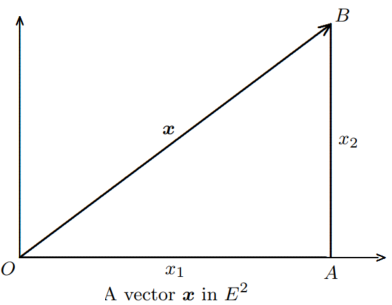
\includegraphics[scale=0.4]{pythagoras.png}
\end{figure}
\end{column}
\end{columns}
\end{itemize}
\end{frame}


\begin{frame}
\frametitle{\: \: \: Scalar Product} 
\toplinemedium
\begin{itemize}
\item Scalar product is a single number that determines the relationship between two vectors of the same dimension:
\begin{eqnarray*}
\langle \bm{x},\bm{y} \rangle=\bm{x}^T \bm{y}=\mathlarger{\sum}_{i=1}^{n}x_i \: y_i
\end{eqnarray*}
where both vectors are of size $nX1$
\vspace{0.11in}
\item Another important property is that if the angle between two vectors, $\theta$, is zero, then:
\begin{columns}
\begin{column}{0.3\linewidth}
\begin{eqnarray*}
\langle \bm{x},\bm{y} \rangle=\|\bm{x}\| \: \|\bm{y}\|
\end{eqnarray*}
\end{column}
\begin{column}{0.7\linewidth}
\begin{itemize}
\item This property is based on multiplying a vector by a scalar: 
\end{itemize}
\begin{figure}
\centering
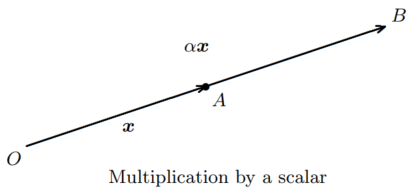
\includegraphics[scale=0.4]{scalar.png}
\end{figure}
\end{column}
\end{columns}
\end{itemize}
\end{frame}


\begin{frame}
\frametitle{\: \: \: Scalar Product} 
\toplinemedium
\begin{itemize}
\item Scalar product is a single number that determines the relationship between two vectors of the same dimension:
\begin{eqnarray*}
\langle \bm{x},\bm{y} \rangle=\bm{x}^T \bm{y}=\mathlarger{\sum}_{i=1}^{n}x_i \: y_i
\end{eqnarray*}
where both vectors are of size $nx1$
\vspace{0.11in}
\item Lastly if the angle between two vectors, $\theta=90^{\circ}$ (i.e. they are \textbf{orthogonal}), then:
\begin{columns}
\begin{column}{0.3\linewidth}
\begin{eqnarray*}
\langle \bm{x},\bm{y} \rangle=0
\end{eqnarray*}
\end{column}
\begin{column}{0.7\linewidth}
\begin{itemize}
\item E.g. $\bm{x}^T=[1,0]$, $\bm{y}^T=[0,1]$
\end{itemize}
\begin{figure}
\centering
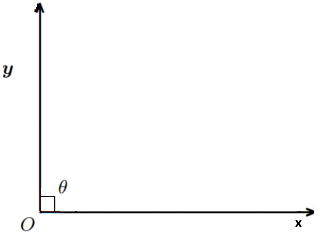
\includegraphics[scale=0.4]{orthogonal.png}
\end{figure}
\end{column}
\end{columns}
\end{itemize}
\end{frame}

\begin{frame}
\frametitle{\: \: \: Vector Addition} 
\toplinemedium
\begin{itemize}
\item Adding two vectors of size $n$ results in:
\begin{columns}
\begin{column}{0.3\linewidth}
\begin{eqnarray*}
\bm{z}=\bm{x}+\bm{y}=\begin{bmatrix}
     x_{1}+y_1  \\
    x_{2}+y_2  \\
     \vdots              \\
    x_{n}+y_n\\
  \end{bmatrix}
  \end{eqnarray*}
 \end{column} 
 \begin{column}{0.7\linewidth}
 \begin{figure}
\centering
\caption{Vector addition in 2 dimensions}
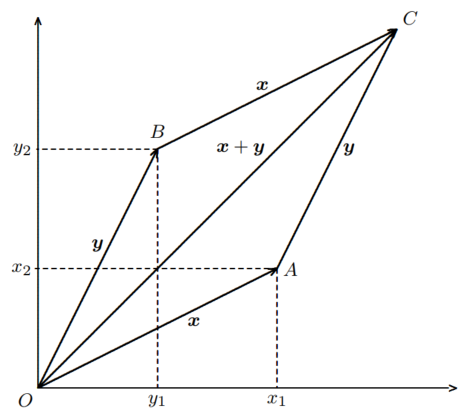
\includegraphics[scale=0.4]{vector_addition.png}
\end{figure}
\end{column}
\end{columns}
\item Vector addition can be combined with multiplication by a scalar 
\end{itemize}
\end{frame}

\begin{frame}
\frametitle{\: \: \: Euclidean Spaces and Subspaces} 
\toplinelarge
\begin{itemize}
\item Vectors of size $n$ can be thought as coordinates of a point in $E^n$
\vspace{0.11in}
\item The minimum set of vectors that spans a particular space are called the \textbf{basis} vectors
\vspace{0.11in}
\begin{itemize}
\item We need $k$ linearly independent vectors of size $n\geq k$ to span the k-dimensional space
\vspace{0.11in}
\item If $k<n$, we call $k$ a subspace of $E^n$
\end{itemize}
\end{itemize}
\end{frame}

\begin{frame}
\frametitle{\: \: \: Orthogonal Complement} 
\toplinelarge
\begin{itemize}
\item We call an orthogonal complement, the set of vectors in $E^n$ that are orthogonal to the basis vectors of a k-dimensional subspace.
\begin{columns}
\begin{column}{0.3\linewidth}
\begin{eqnarray*}
\langle \bm{x},\bm{z} \rangle=0
\end{eqnarray*}
 \end{column} 
 \begin{column}{0.7\linewidth}
 \begin{figure}
\caption{Example with $n=2$, $k=1$}
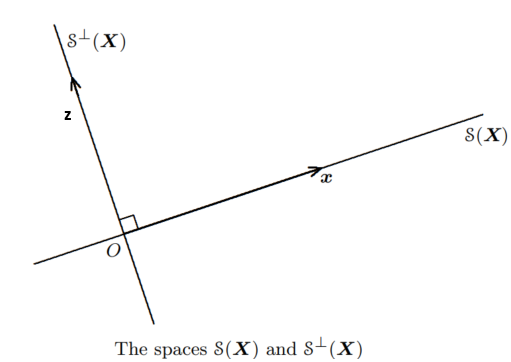
\includegraphics[scale=0.4]{orth.png}
\end{figure}
\end{column}
\end{columns}
\item These vectors live in the $n-k$ space
\end{itemize}
\end{frame}

\begin{frame}
\frametitle{\: \: \: Linear Regression} 
\toplinelarge
\begin{itemize}
\item Linear Regression considers each linearly-independent $k$ column vector of size $n$ from $\bm{X}$ as the basis vector that spans the k-dimensional space
\begin{itemize}
\vspace{0.11in}
\item We also assume the following two conditions:
\begin{eqnarray*}
\begin{array}{lll}
\bm{X}^T \bm{\hat{u}}=\bm{0} &,   & \bm{y}=\bm{X} \bm{\hat{\beta}}+\bm{\hat{u}}
\end{array}
\end{eqnarray*}
\item This result in linear regression being defined as selecting $\bm{\hat{\beta}}$ that reaches the perpendicular dropped from $\bm{y}$ vector into the plane spanned by $\bm{X}$  
\end{itemize}
\end{itemize}
\end{frame}

\begin{frame}
\frametitle{\: \: \: Linear Regression} 
\toplinelarge
 \begin{figure}
\caption{Example with $n=3$, $k=2$}
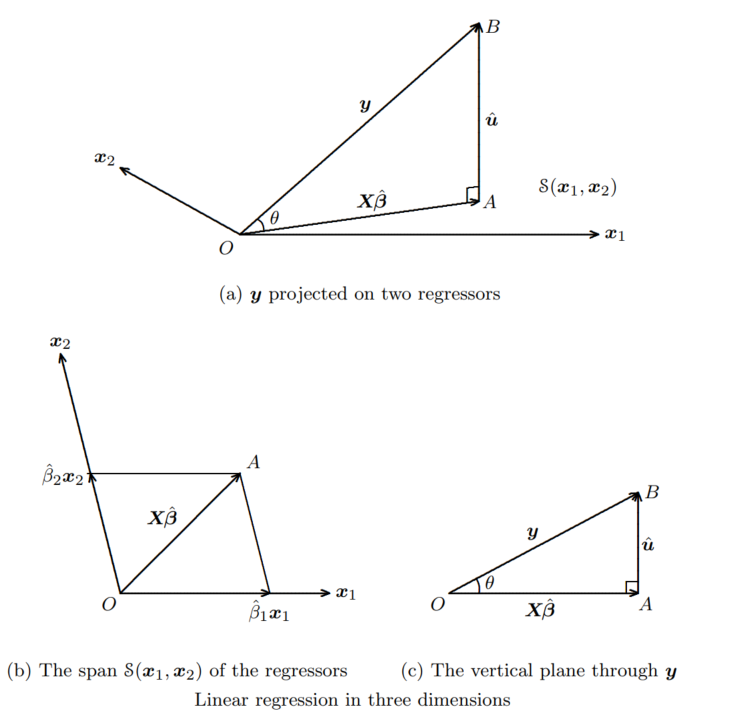
\includegraphics[scale=0.34]{linear_regression.png}
\end{figure}
\end{frame}

\end{document}